
\textbf{Experimental Setup.}
We implement our deep reasoning model (DRM) using \textsc{tensorflow-1.4.0} and \textsc{Keras-2.0.8}. To implement CNNs, we use rectified linear units (relu) as activation functions and 300 convolutional filters with windows size of 2. We train the model with Adam optimizer with start learning rate $0.001$. We adopt \emph{accuracy} as our main evaluation metric, which measures how many selected text spans contain the answer out of all. The following  methods are compared:\\
% \begin{itemize}
% \vspace{-1mm}
% \setlength\itemsep{-0.8mm}
$\bullet$ \textbf{DRM-type 1} and \textbf{DRM-type 2} Our deep reasoning models with type 1 /type 2 action. \\
% $\bullet$  \textbf{DRM-type 2} Our deep reasoning model with type 2 action, as described in Section \ref{sec:design}. \\
$\bullet$  \textbf{DRM-type 2 w/ human} We consider a variant of our deep reasoning model with human in the loop, in order to demonstrate that our model has the ability to interact with humans. At each decision step, if the algorithm's confidence in its best action is lower than a pre-specified threshold $T_r=0.6$, the algorithm asks a human to pick an action from the $2\times k$ actions. We assume that humans always make the right decision w.r.t. the ground truth.  \\
$\bullet$  \textbf{DRM-noRL} We test our model structure with multi-class classification loss. Each segment is assigned a score, and the segment with the highest score is predicted. \\
 $\bullet$  \textbf{Gradient Boosting}. 
 % A  binary classifier to evaluate different (question, context segment) pairs and select the segment with the highest prediction score. corollary
% Bag-of-words features are first extracted separately from both the question and the segment and then concatenated. We choose Gradient Boosting due to its effectiveness in modeling feature interactions;
Two variants of Gradient Boosting are tested, one trained with binary cross entropy loss, and the other with ranking loss. In addition to bag-of-words features, for fairness we introduce four new discourse features: left and right discourse markers, the position of the target word, the first word of the question.\\
$\bullet$  \textbf{BM25} We use BM25~\cite{DBLP:journals/ftir/RobertsonZ09} as a bag-of-words retrieval function to rank segments based on the question terms. \\
%$\bullet$  \textbf{Chunked BoW Model}~\cite{DBLP:conf/acl/ChoiHUPLB17}. This is similar to the Gradient Boosting-binary model, except that the binary classifier employed is a neural network with fully connected layers. \\
$\bullet$  \textbf{Coarse-to-Fine Answer Selector}~\cite{DBLP:conf/acl/ChoiHUPLB17} concatenates the context and the question, and run a neural network on it to select the relevant text span. We adopt their Chunked BoW setup.\\
$\bullet$  \textbf{RaSoR}~\cite{DBLP:journals/corr/LeeKP016} builds a deep neural network model to select a span of text as the answer. Each candidate span is fixed-length representated using BiLSTM and neural co-attention. 
% \end{itemize}

\subsection{Experimental Results}
%0. RL learning curve\\




We report the overall segment prediction accuracy on the datasets and the accuracy on each question type (Table~\ref{tab:main}). On both QAMR dataset and PTB dataset, DRM-type 2 with human in the loop achieves the highest accuracy. Being able to interact with humans is an advantage of our approach; 
% Humans can understand the decision process of the algorithm and can intervene if necessary. By contrast, 
none of the competitor approaches can do this, either because their decision process is a single-step process or because their decision process is not interpretable. In our experiment, 65\% QA pairs (less than the threshold) get help from human at one reasoning step, and their performance increases 0.15. It is also very interesting to learn that the remaining 35\% data points with high confidence reasoning learned by our model perform 0.06 better than the average performance. To further understand whether the improvement comes from human's selection or from our model's judgement, we allow the model to randomly select 65\% of the QA pairs, and for each pair, to interact with human once without considering their confidence. The results show that such random selection procedure doesn't make any difference on performance. Even without human's help, our DRM-type 2 model still achieves better performance than all other methods. As expected, DRM-type 2 model performs better than DRM-type 1 model, since type 2 actions leverage more information. 
%Looking at how the algorithm performs as the number of reasoning steps increases, the prediction accuracy increases slightly as the reasoning gets longer: the accuracy for 1-step, 2-step, 3-step and 4-step reasoning is 0.700,0.700,0.705 and 0.727.

Among the baseline methods, Gradient Boosting trained on both bag-of-words + discourse features works best. These models perform much worse if trained only on bag-of-words features. This shows that the structure/order information captured by discourse features is essential, which Neural network doesn't do. 
% The classical BM25 works well on questions that start with ``whose" but terribly on questions that start with ``why". 
Since BM25 solely relies on similarity between the question and the segment, it only works well when the the question and the correct segment have many overlapping words, as in the case of ``whose" questions, but not ``why" questions.

We also study whether the learned reasoning model is transferable by training DRM on the QAMR dataset but test the learned model on PTB dataset. Results in Table~\ref{tab:main} show that this model generalizes well on PTB dataset -- its performance is very close to the DRM model trained on PTB directly. We also observe that the RaSoR model achieves a very good performance. We think this is because training a deep neural network model benefits from the larger number of training samples in QAMR dataset. 


\subsection{Comparison with QA Methods}
In this section, we compare our model with several other benchmark QA models on the QAMR and PTB datasets. The results are shown in Table~\ref{tab:nnresults}. 
\begin{table}[h]
	\centering
	\resizebox{0.8\columnwidth}{!}{%resize the table
\begin{tabular}{|l|c|c|}
  \hline
  \textsc{Model} & \textsc{QAMR} & \textsc{PTB}   \\
  \hline
  MemNets & .476 & .423 \\
  GA-Reader (fix $L(w)$) & .610 & .532 \\
  QANet & .703 & .602   \\
  Mnemonic Reader & .700 & .595 \\
  DRM-type 2 & .702 & .599   \\
  \hline
\end{tabular}
}
\caption{\fontsize{10}{12}\selectfont  Our model vs. popular QA models.}\label{tab:nnresults}
  \vspace{-2ex}
\end{table}
Most of these approaches are originally designed to extract the exact answer(s) from the context. In order to modify these models' outputs as a segment, we change the training target from the exact answer to an answer segment. We observe that QANet gives the best accuracy in terms of selecting the correct text span containing the answer. 
% All these methods except QANet can be considered as multi-step reasoning models, and our model gives the best performance among all these models.
% 1. discourse is better than no discourse in Gradient Boosting and Gradient Boostingrank
% 2. bm25 model similarity, perform not very well e.g. 'The victory comes (after) a few days (because)blabla' What comes a few days after?
% 3. bow and cnn can't explicitly model discourse info, so perform not very well
% 4. compare two setups? binary classifier vs. pairwise ranking
% 3. drmtype2 perform better than drmtype1 as we expected
% 4. introduce how human-in-the-loop work
% 5. 
% 6. compare drm-transfer and drm-ptb: why better than ptb why because ptd does not contain many why question.


%Because the deep reasoning model appear to capture high-level information about context structures, we hypothesize that the models should perform very well even when training on data from different domains. http://www.aclweb.org/anthology/P14-1092


\begin{table*}[t]
\centering
{
	\fontsize{9}{9}\selectfont
  %\setlength{\baselineskip}{0pt}
  \setlength{\tabcolsep}{1.0mm}
  \renewcommand{\arraystretch}{1.1}
	%\hspace{4mm}
	\begin{tabular}{|p{1.8cm}|p{2.5cm}|p{2.5cm}|p{2.5cm}|p{5.8cm}|}
 	\hline
 	\textbf{Question genre}  & \textbf{Same side}& \textbf{Opposite sides}& \textbf{Context-dependent (side)} &  \textbf{Example QA pairs} \\
 	\hline
 	when \newline what year \newline how long 
 	& \textbf{step 1}: already, again, still, following \newline\textbf{step 2}: while, yet & \textbf{step 1}: as soon as, at that \newline\newline \textbf{step 2}: then, further, originally
 	&\textbf{step 1}: previously, until, back, after, soon, during \newline \textbf{step 2}: since, second, next, when, as well, because, who 
	&  \textbf{Context: }28 \textit{\textcolor{blue}{skiers}} earned DNFs \textit{\textcolor{red}{during}} \underline{the first run}, \textit{\textcolor{red}{and}} nine earned DNFs \textit{\textcolor{red}{during}} their second runs.
  \newline \textbf{Question: }When did \textit{\textcolor{blue}{skiers}} earn DNFs? 
  \newline \textbf{Learned Reasoning: } during-right, and-left\\ 
	\hline
  why \newline what caused 
 &\textbf{step 1}: in order to, because, due to,  since \newline\textbf{step 2}: as, but &\textbf{step 1}: at that, previously, though, if, since \newline \textbf{step 2}: second, for, to, or, that, not, and & \textbf{step 1}: well, following, initially  \newline\newline\textbf{step 2}: which, even,certainly  
  & \textbf{Context: }Given its initial condition, prediction of its final condition is possible, causally \textit{\textcolor{red}{but}} only probabilistically, \textit{\textcolor{red}{because}} the Schrödinger equation is deterministic for wave function evolution, \textit{\textcolor{red}{but}} \underline{the wave function describes the system only} \underline{\textit{\textcolor{blue}{probabilistically}}}.
  \newline \textbf{Question: }Why is the prediction \textit{\textcolor{blue}{probabilistic}}?
  \newline \textbf{Learned Reasoning: }because-right, but-right\\ 
	\hline	
	who+past tense 

	& \textbf{step 1}: rather, thus, including \newline\newline\textbf{step 2}: nor, who, initially &\textbf{step 1}: earlier, definitely, previously \newline\newline\textbf{step 2}: particularly, seemingly
		&\textbf{step 1}: ultimately, since, when, later, while, finally \newline \textbf{step 2}:  again, last, and , after, next, 
	& \textbf{Context: }\underline{Hatch had} \textit{\textcolor{red}{previously}} \textit{\textcolor{blue}{survived}} a separate crash in 2003, \textit{\textcolor{red}{that}} killed his mother, brother \textit{\textcolor{red}{and}} sister.
  \newline \textbf{Question: }Who \textit{\textcolor{blue}{survived}}?\newline \textbf{Learned Reasoning: }previously-left\\ 
	\hline
  where 
 
  
	 &\textbf{step 1}: following, to explain, while \newline\newline\textbf{step 2}: possibly, initially, finally, hence &\textbf{step 1}: to, before, back, in that, eventually \newline\textbf{step 2}: like, or, as & \textbf{step 1}: in which, then, second, next \newline\newline \textbf{step 2}: too, yet, second, including, after, next
  & \textbf{Context: }\textit{\textcolor{red}{Once}} the proposed \textit{\textcolor{blue}{amendment}} has passed those hurdles, \textit{\textcolor{red}{then}} the amendment goes \textit{\textcolor{red}{to}} \underline{Indiana voters} \textit{\textcolor{red}{who}} vote yea or nay on the amendment. 
  \newline \textbf{Question: }Where does the \textit{\textcolor{blue}{amendment}} go?
  \newline \textbf{Learned Reasoning: }to-right, who-left\\ 
 \hline
\end{tabular}
}
\caption{\fontsize{9}{12}\selectfont Top discourse markers are associated with question genres, and focus direction is learned in \textsc{QAMR} dataset. We show four different question genres: time, reason, person, and location.}
\label{tab:disc_phrase}
\vspace{-3ex}
\end{table*}

Our method has an obvious advantage over the others: unlike the multi-step models where the number of steps need to be predefined, our model is capable of using a dynamic number of reasoning steps to resolve different QA pairs. Another very important difference is that the existing models achieve multi-step by updating the internal vector representations, which is not interpretable, while our model directly prunes the context for an interpretable reasoning process.

\subsection{Experiment on SQuAD}

\begin{figure}
 \centering
 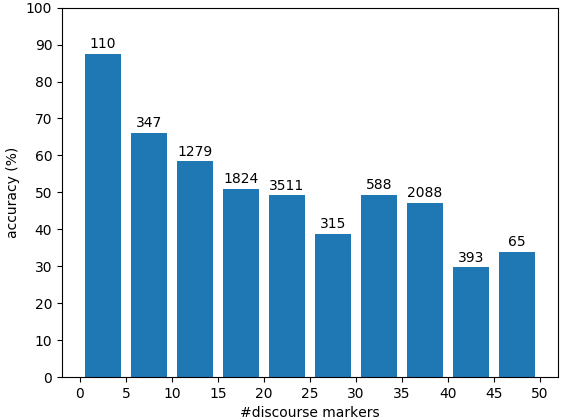
\includegraphics[width=0.9\linewidth]{fig/squad.png}
 \caption{\kechen{Accuracy on each discourse marker interval of SQuAD dataset, which contains 10,570 documents. We show the number of documents in each interval on top of each bar.}}
 \label{fig:squad}
\vspace{-2ex}
\end{figure}

\kechen{1. can we say small \#dm indicates short context  2.bert on squad solve a harder task, how do we compare our result with them.} We next experiment our method on the SQuAD dataset. To show the performance on different context size, we group documents into buckets based on the number of discourse markers they contain, and report the model performance of each bucket. Experimental results show that the performance on short context (\emph{e.g.} $<$5 discourse markers) is comparable to state-of-the-art single BERT model \cite{DBLP:journals/corr/abs-1810-04805}, but the performance drop a lot when the number of discourse markers increase. We think excessive number of discourse markers in long document tends to give redundant reasoning steps. Binary searching by discourse markers in such long documents is not necessarily how human read and interpret long expositions, so our method is less applicable. In long context scenarios, we suppose one can use coarse-to-fine strategy to pinpoint the answer in a relatively short span, and then apply our approach to infer the reasoning path and the answer. To verify our speculation, we simulate coarse-to-fine step by selecting a short text span around the labeled answer. The extracted text spans contain 5.7 discourse markers in average and serve as new context. We then apply our model on it to predict the answer segment. Experimental results show that the overall accuracy on whole SQuAD dev dataset is 0.82. This new result is much better than it on original dataset and comparable to STOA result. 